
\begin{figure*}[h!]
\begin{subfigure}[t]{.5\textwidth}
   \centering
    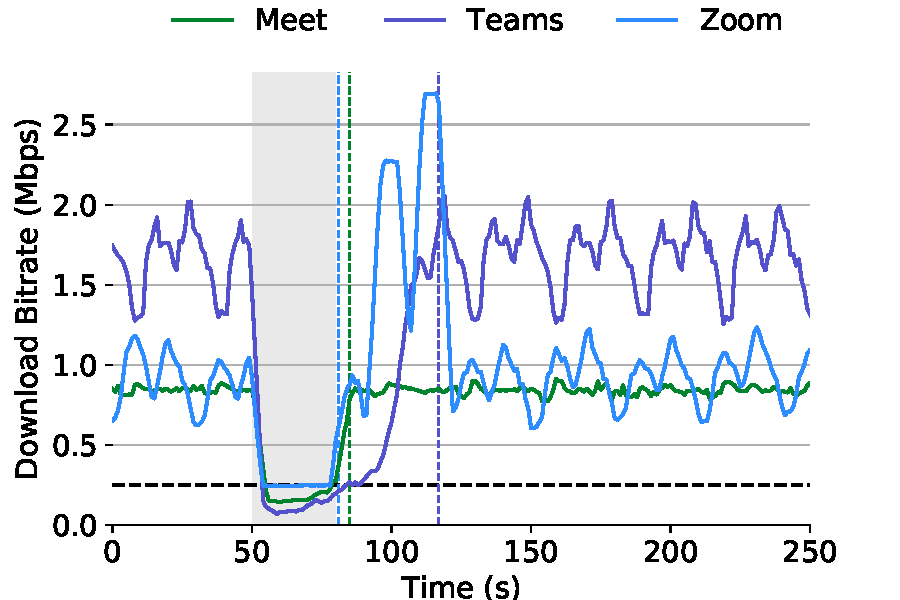
\includegraphics[width=1\textwidth,keepaspectratio]{interrupt/Interrupt-dnld.pdf}
    \captionsetup{width=.9\linewidth}
    \caption{Average downlink bitrate over time. Grey region indicates period where downlink capacity is constrained to 0.25 Mbps. Vertical dotted lines indicate when the dowlink bitrate has returned to the average. Dotted horizontal line indicates the downlink shaping level.}
    \label{fig:ts-dnld}
\end{subfigure}
\begin{subfigure}[t]{.5\textwidth}
  \centering
    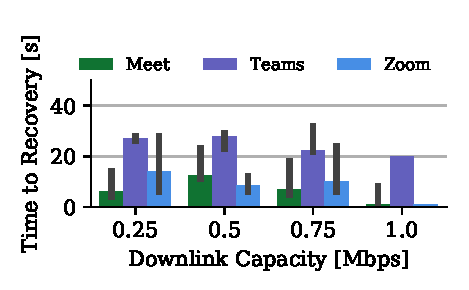
\includegraphics[width=1\textwidth,keepaspectratio]{../figures/interrupt/TTR-dnld.pdf}
    \captionsetup{width=.9\linewidth}
    \caption{The time to recover to average receiving bitrate following a drop to the indicated downlink shaping level}
    \label{fig:TTR_dnld}
\end{subfigure}
\caption{VCA response to a 30s drop in available downlink capacity}
\label{fig:interrupt-dnld}
\end{figure*}

\section{Temporary Interruptions}
\label{sec:interruption}

In this section, we discuss how VCAs respond to temporary bandwidth drops during the call. Using the same setup as Figure \ref{fig:static_setup}, a 5 minute VCA call is initiated between two clients, C1 and C2, both of which sit behind unconstrained links. Once the VCA reaches its nominal consumption, we reduce the available bandwidth between C1 and the router for 30 seconds, before reverting back to an unconstrained link. We conduct two sets of experiments, shaping the uplink in the fist and the downlink in the second. We consider the following shaping levels: {0.25, 0.5, 0.75, 1.0} Mbps. We don't shape beyond 1.0 Mbps because both Zoom and Meet's average bitrate is below 1.0 Mbps.


\subsection{Uplink Shaping}
Focusing first on uplink shaping, Figure \ref{fig:ts_upld} illustrates VCA uplink bitrate over the course of a call. It is clear that the path to recovery and the time to recovery following the interruption differ greatly among the VCAs. In order to compare the recovery times of each VCA, we introduce a metric called \textit{time to recovery} (TTR). We define TTR as the time between when the interruption ends and when the 5 second rolling median bitrate reaches the average bitrate. In other words, how long it takes the VCA performance to return to normal following the interruption. Figure \ref{fig:TTR_upld} shows how the uplink shaping level affects each VCA's time to recovery. There is a clear trend that the more severe the upload shaping, the longer the VCAs need to recover. This trend, however, is less pronounced for Teams than it is for Meet and Zoom because Teams takes longer to recovery at less severe shaping levels. Teams's slow recovery is explained by the recovery trend in Figure \ref{fig:ts_upld}. Teams follows a cubic trendline, slowing increasing the uplink bitrate immediately after the interruption before increasing quickly back to normal. Meet also observes this cubic recovery at the 0.25 Mbps shaping level but recovers much faster otherwise. 

While Meet and Teams seem to follow a cubic trendline, Zoom's recovery is markedly different. Looking at Figure \ref{fig:ts_upld}, Zoom follows a stepwise recovery, slowly increases the sending bitrate, then going well above the nominal rate, before finally dropping back to the average bitrate. Zoom does not return to a ``normal'' sending pattern until 2 minutes after the interruption, sending at much higher rates than necessary. It is possible that this inefficient uses of the uplink could disturb other applications on the same link, leading to a poor quality of experience for competing applications. 

\subsection{Downlink Shaping}
Turning now to downlink shaping, it is clear that Teams recovers much slower than Meet and Zoom, always taking at least 20 seconds longer to return to the average rate, regardless of the magnitude of the interruption. This can be explained by the way each VCA sends video. In all three VCAs, C1 and C2 communicate through an intermediary server. Meet uses an encoding technique called \textit{simulcast}, where the client encodes two versions ~\cite{nistico2020comparative}. The server then sends the appropriate version based on the perceived downlink capacity at the receiver. This way, a sender transmitting on an unconstrained link does not have to adjust its sending and can rely on the server to send the appropriate version. The server can then quickly switch between which version to send to the receiver based on the feedback it receives. This quick recovery is clearly illustrated in \ref{fig:interrupt-dnld}, in which Meet returns to its nominal rate in under 10 seconds, depending on the severity of the interruption.

Similarly, Zoom uses \textit{multi-bitrate encoding} when transmitting video~\cite{zoom_encoding}. Instead of sending several versions of varying quality, Zoom sends many "layers" that, when superimposed, produce a high quality video. This allows C2 to continue sending uninterrupted even when C1's downlink capacity shrinks. 

\begin{figure}[t]
    \centering
    \includegraphics[width=0.45\textwidth,keepaspectratio]{../figures/interrupt/Interrupt-sender.pdf}
    \caption{Client 2 (C2) uplink bitrate. Grey region indicates when C1's downlink capacity is reduced to 0.25 Mbps}
    \label{fig:interrupt-sender}
\end{figure}

While the intermediary server for Zoom and Meet does congestion control, it only acts as a relay for Teams. During a Teams call, C2 will recognize C1 has limited downlink capacity and adjust its behavior, sending at only the bitrate it knows C1 can handle. Once C1 has more available bandwidth, however, C2 must first probe the connection before returning to its nominal sending rate. Figure \ref{fig:interrupt-sender} illustrates how C2's sending rate does not change during a Meet call, but drops below the shaping threshold during a Teams call, leading to the slow recovery.

In terms of how efficiently each VCA uses the constrained link, Zoom's downlink and uplink bitrate stays at the shaping level while Meet and Teams fall even lower than the shaping level. 

\noindent \textbf{Takeaways}: The observed VCA responses to interruptions portend even greater recovery times on real home networks. Greater fluctuations in link capacity will lead to frequent interruptions. While all VCAs take close to 20 seconds to recover from severe drops in available bandwidth, Teams consistently requires at least 20 seconds to recover from even moderate drops to 1 Mbps to either the uplink or the downlink.






